\documentclass[english, twocolumn, 10pt, aps, superscriptaddress, floatfix, prb, citeautoscript]{revtex4-1}
\pdfoutput=1
\usepackage[utf8]{inputenc}
\usepackage[T1]{fontenc}
\usepackage{listings}
\usepackage{units}
\usepackage{mathtools}
\usepackage{amsmath}
\usepackage{amssymb}
\usepackage{graphicx}
\usepackage{wasysym}
\usepackage{layouts}
\usepackage{siunitx}
\usepackage{bm}
\usepackage{xcolor}
\usepackage[colorlinks, citecolor={blue!50!black}, urlcolor={blue!50!black}, linkcolor={red!50!black}]{hyperref}
\usepackage{bookmark}
\usepackage{tabularx}
\usepackage{microtype}
\usepackage{babel}
\usepackage{textcomp}
\hypersetup{pdfauthor={Tinkerer},pdftitle={Adaptive, tools for adaptive parallel sampling of mathematical functions}}

\setcounter{secnumdepth}{4}
\setcounter{tocdepth}{4}

\DeclareMathOperator{\e}{e}
\DeclareMathOperator{\de}{d\!}
\DeclareMathOperator{\Tr}{Tr}
\DeclareMathOperator{\diag}{diag}
\DeclareMathOperator{\Res}{Res}
\DeclareMathOperator{\sgn}{sgn}
\DeclareMathOperator{\Pf}{Pf}
\DeclareMathOperator{\Det}{Det}
\DeclareMathOperator{\rank}{rank}
\DeclareMathOperator{\im}{Im}
\DeclareMathOperator{\re}{Re}
\newcommand{\kx}{k_x}
\newcommand{\ky}{k_y}
\newcommand{\meff}{m_\text{eff}}
\newcommand{\R}{\mathbb{R}}

\newcounter{CommentNumber}
% \renewcommand{\paragraph}[1]{\stepcounter{CommentNumber}\belowpdfbookmark{#1}{\arabic{CommentNumber}}}

\DeclarePairedDelimiter\abs{\lvert}{\rvert}
\DeclarePairedDelimiter\norm{\lVert}{\rVert}

\makeatletter
\let\oldabs\abs
\def\abs{\@ifstar{\oldabs}{\oldabs*}}
\let\oldnorm\norm
\def\norm{\@ifstar{\oldnorm}{\oldnorm*}}
\makeatother

\newcommand{\ev}[1]{\langle#1\rangle}
\newcommand{\bra}[1]{\langle#1|}
\newcommand{\ket}[1]{|#1\rangle}
\newcommand{\bracket}[2]{\langle#1|#2\rangle}

\newcolumntype{L}[1]{>{\raggedright\arraybackslash}p{#1}}
\newcolumntype{C}[1]{>{\centering\arraybackslash}p{#1}}
\newcolumntype{R}[1]{>{\raggedleft\arraybackslash}p{#1}}

% workaround for https://github.com/jgm/pandoc/issues/2392#issuecomment-140114736
\renewcommand{\citep}{\cite}

% workaround for https://github.com/jgm/pandoc/issues/4716
\newcommand{\passthrough}[1]{\lstset{mathescape=false}#1\lstset{mathescape=true}}

% listing settings, from https://tex.stackexchange.com/a/179956
\lstset{
    basicstyle=\ttfamily,
    numbers=left,
    keywordstyle=\color[rgb]{0.13,0.29,0.53}\bfseries,
    stringstyle=\color[rgb]{0.31,0.60,0.02},
    commentstyle=\color[rgb]{0.56,0.35,0.01}\itshape,
    numberstyle=\footnotesize,
    stepnumber=1,
    numbersep=5pt,
    backgroundcolor=\color[RGB]{248,248,248},
    showspaces=false,
    showstringspaces=false,
    showtabs=false,
    tabsize=2,
    captionpos=b,
    breaklines=true,
    breakatwhitespace=true,
    breakautoindent=true,
    escapeinside={\%*}{*)},
    linewidth=\columnwidth,
    basewidth=0.5em,
}


\begin{document}

\title{Adaptive, tools for adaptive parallel sampling of mathematical functions}

\author{Tinkerer}
\email[Electronic address: ]{not\_anton@antonakhmerov.org}
\affiliation{Kavli Institute of Nanoscience, Delft University of Technology, P.O. Box 4056, 2600 GA Delft, The Netherlands}

\date{\today}

\begin{abstract}
Large scale computer simulations are time-consuming to run and often require sweeps over input parameters to obtain a qualitative understanding of the simulation output.
These sweeps of parameters can potentially make the simulations prohibitively expensive.
Therefore, when evaluating a function numerically, it is advantageous to sample it more densely in the interesting regions (called adaptive sampling) instead of evaluating it on a manually-defined homogeneous grid.
Such adaptive algorithms exist within the machine learning field.
These mehods can suggest a new point to calculate based on \textit{all} existing data at that time; however, this is an expensive operation.
An alternative is to use local algorithms---in contrast to the previously mentioned global algorithms---which can suggest a new point, based only on the data in the immediate vicinity of a new point.
This approach works well, even when using hundreds of computers simultaneously because the point suggestion algorithm is cheap (fast) to evaluate.
We provide a reference implementation in Python and show its performance.
\end{abstract}

\flushbottom
\maketitle

\hypertarget{introduction}{%
\section{Introduction}\label{introduction}}

\hypertarget{simulations-are-costly-and-often-require-sampling-a-region-in-parameter-space.}{%
\paragraph{Simulations are costly and often require sampling a region in parameter space.}\label{simulations-are-costly-and-often-require-sampling-a-region-in-parameter-space.}}

In the computational sciences, one often does costly simulations---represented by a function \(f\)---where a certain region in parameter space \(X\) is sampled, mapping to a codomain \(Y\): \(f \colon X \to Y\).
Frequently, the different points in \(X\) can be independently calculated.
Even though it is suboptimal, one usually resorts to sampling \(X\) on a homogeneous grid because of its simple implementation.

\hypertarget{choosing-new-points-based-on-existing-data-improves-the-simulation-efficiency.}{%
\paragraph{Choosing new points based on existing data improves the simulation efficiency.}\label{choosing-new-points-based-on-existing-data-improves-the-simulation-efficiency.}}

An alternative, which improves the simulation efficiency, is to choose new potentially interesting points in \(X\), based on existing data \citep{Gramacy2004, Figueiredo1995, Castro2008, Chen2017}.
Bayesian optimization works well for high-cost simulations where one needs to find a minimum (or maximum) \citep{Takhtaganov2018}.
However, if the goal of the simulation is to approximate a continuous function using the fewest points, the continuity of the approximation is achieved by a greedy algorithm that samples mid-points of intervals with the largest distance or curvature \citep{Wolfram2011}.
Such a sampling strategy (i.e., in Fig.~\ref{fig:algo}) would trivially speedup many simulations.
Here, the complexity arises when parallelizing this algorithm, because this requires a lot of bookkeeping and planning.

\begin{figure}
\hypertarget{fig:algo}{%
\centering
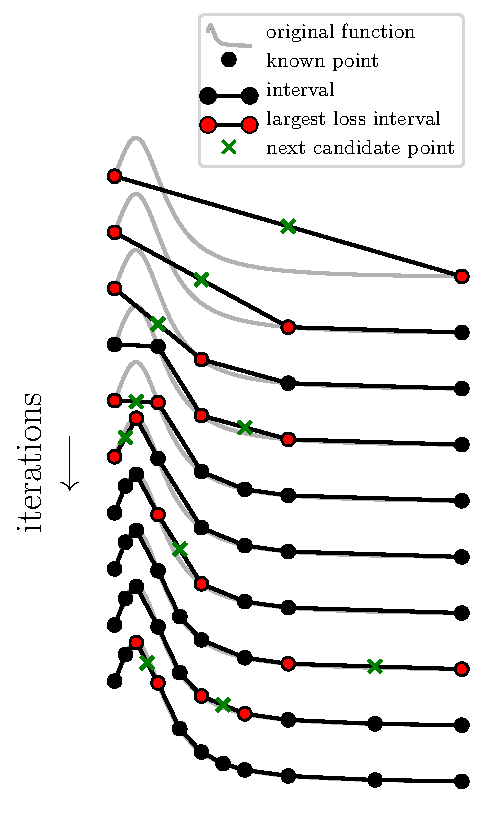
\includegraphics{figures/algo.pdf}
\caption{Visualization of a 1-D point choosing algorithm for a black box function (grey).
We start by calculating the two boundary points.
Two consecutive existing data points (black) \(\{x_i, y_i\}\) define an interval.
Each interval has a loss \(L_{i,i+1}\) associated with it that can be calculated from the points inside the interval \(L_{i,i+1}(x_i, x_{i+1}, y_i, y_{i+1})\) and optionally of \(N\) next nearest neighbouring intervals.
At each iteration the interval with the largest loss is indicated (red), with its corresponding candidate point (green) picked in the middle of the interval.
The loss function in this example is the curvature loss.}\label{fig:algo}
}
\end{figure}

\hypertarget{we-describe-a-class-of-algorithms-relying-on-local-criteria-for-sampling-which-allow-for-easy-parallelization-and-have-a-low-overhead.}{%
\paragraph{We describe a class of algorithms relying on local criteria for sampling, which allow for easy parallelization and have a low overhead.}\label{we-describe-a-class-of-algorithms-relying-on-local-criteria-for-sampling-which-allow-for-easy-parallelization-and-have-a-low-overhead.}}

To handle many parallel workers that calculate the function values and request new points, the algorithm needs to have a low computational overhead.
Requiring that, when a new point has been calculated, that the information updates are local (only in a region around the newly calculated point), will reduce the time complexity of the algorithm.
A simple example is greedily optimizing continuity of the sampling by selecting points according to the distance to the largest gaps in the function values, as in Fig.~\ref{fig:algo}.
For a one-dimensional function with three points known (its boundary points and a point in the center), such a simple algorithm consists of the following steps:
(1) keep all points \(x\) sorted, where two consecutive points define an interval,
(2) calculate the distance for each interval \(L_{i, i+1}=\sqrt{(x_{i+1}-x_{i})^{2}+(y_{i+1}-y_{i})^{2}}\),
(3) pick a new point \(x_\textrm{new}\) in the middle of the interval with the largest \(L\), creating two new intervals around that point,
(4) calculate \(f(x_\textrm{new})\),
(5) repeat the previous steps, without redoing calculations for unchanged intervals.

In this paper, we present a class of algorithms that rely on local criteria for sampling, such as in the former example.
Here we associate a \emph{local loss} to each interval and pick a \emph{candidate point} inside the interval with the largest loss.
For example, in the case of the integration algorithm, the loss is the error estimate.
The advantage of these \emph{local} algorithms is that they allow for easy parallelization and have a low computational overhead.

\begin{figure}
\hypertarget{fig:Learner1D}{%
\centering
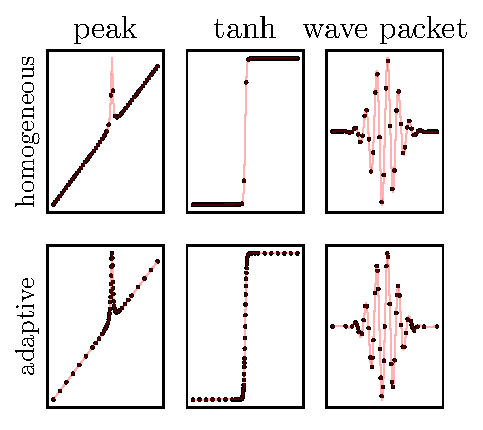
\includegraphics{figures/Learner1D.pdf}
\caption{Comparison of homogeneous sampling (top) with adaptive sampling (bottom) for different one-dimensional functions (red) where the number of points in each column is identical.
We see that when the function has a distinct feature---such as with the peak and tanh---adaptive sampling performs much better.
When the features are homogeneously spaced, such as with the wave packet, adaptive sampling is not as effective as in the other cases.}\label{fig:Learner1D}
}
\end{figure}

\begin{figure}
\hypertarget{fig:Learner2D}{%
\centering
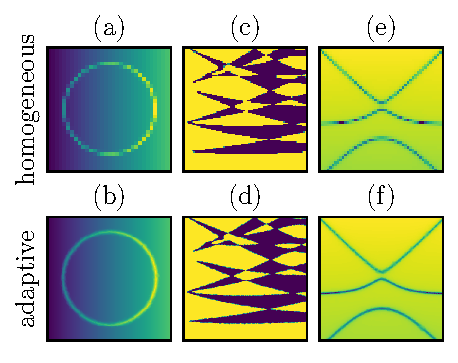
\includegraphics{figures/Learner2D.pdf}
\caption{Comparison of homogeneous sampling (top) with adaptive sampling (bottom) for different two-dimensional functions where the number of points in each column is identical.
On the left is the function \(f(x) = x + a ^ 2 / (a ^ 2 + (x - x_\textrm{offset}) ^ 2)\).
In the middle a topological phase diagram from \onlinecite{Nijholt2016}, where the function can take the values -1 or 1.
On the right we plot level crossings for a two level quantum system.
In all cases using Adaptive results in a higher fidelity plot.}\label{fig:Learner2D}
}
\end{figure}

\hypertarget{we-provide-a-reference-implementation-the-adaptive-package-and-demonstrate-its-performance.}{%
\paragraph{We provide a reference implementation, the Adaptive package, and demonstrate its performance.}\label{we-provide-a-reference-implementation-the-adaptive-package-and-demonstrate-its-performance.}}

We provide a reference implementation, the open-source Python package called Adaptive \citep{Nijholt2019}, which has previously been used in several scientific publications \citep{Vuik2018, Laeven2019, Bommer2019, Melo2019}.
It has algorithms for \(f \colon \mathbb{R}^N \to \mathbb{R}^M\), where \(N, M \in \mathbb{Z}^+\) but which work best when \(N\) is small; integration in \(\mathbb{R}\); and the averaging of stochastic functions.
Most of our algorithms allow for a customizable loss function with which one can adapt the sampling algorithm to work optimally for different classes of functions.
It integrates with the Jupyter notebook environment as well as popular parallel computation frameworks such as \passthrough{\lstinline!ipyparallel!}, \passthrough{\lstinline!mpi4py!}, and \passthrough{\lstinline!dask.distributed!}.
It provides auxiliary functionality such as live-plotting, inspecting the data as the calculation is in progress, and automatically saving and loading of the data.

The raw data and source code that produces all plots in this paper is available at \citep{papercode}.

\hypertarget{sec:review}{%
\section{Review of adaptive sampling}\label{sec:review}}

Optimal sampling and planning based on data is a mature field with different communities providing their own context, restrictions, and algorithms to solve their problems.
To explain the relation of our approach with prior work, we discuss several existing contexts.
This is not a systematic review of all these fields, but rather, we aim to identify the important traits and design considerations.

\hypertarget{experiment-design-uses-bayesian-sampling-because-the-computational-costs-are-not-a-limitation.}{%
\paragraph{Experiment design uses Bayesian sampling because the computational costs are not a limitation.}\label{experiment-design-uses-bayesian-sampling-because-the-computational-costs-are-not-a-limitation.}}

Optimal experiment design (OED) is a field of statistics that minimizes the number of experimental runs needed to estimate specific parameters and, thereby, reduce the cost of experimentation \citep{Emery1998}.
It works with many degrees of freedom and can consider constraints, for example when the sample space contains regions that are infeasible for practical reasons.
One form of OED is response-adaptive design \citep{Hu2006}, which concerns the adaptive sampling of designs for statistical experiments.
Here, the acquired data (i.e.~the observations) are used to estimate the uncertainties of a certain desired parameter.
It then suggests further experiments that will optimally reduce these uncertainties.
In this step of the calculation Bayesian statistics is frequently used.
Bayesian statistics naturally provides tools for answering such questions; however, because it provides closed-form solutions, Markov chain Monte Carlo (MCMC) sampling is the standard tool for determining the most promising samples.
In a typical non-adaptive experiment decisions on which experiments to perform, are made in advance.

\hypertarget{plotting-and-low-dimensional-integration-uses-local-sampling.}{%
\paragraph{Plotting and low dimensional integration uses local sampling.}\label{plotting-and-low-dimensional-integration-uses-local-sampling.}}

Plotting a low dimensional function in between bounds requires one to evaluate the function on sufficiently many points such that when we interpolate values in between data points, we get an accurate description of the function values that were not explicitly calculated.
In order to minimize the number of function evaluations, one can use adaptive sampling routines.
For example, for one-dimensional functions, Mathematica \citep{WolframResearch} implements a \passthrough{\lstinline!FunctionInterpolation!} class that takes the function, \(x_\textrm{min}\), and \(x_\textrm{max}\), and returns an object that samples the function more densely in regions with high curvature; however, details on the algorithm are not published.
Subsequently, we can query this object for points in between \(x_\textrm{min}\) and \(x_\textrm{max}\), and get the interpolated value, or we can use it to plot the function without specifying a grid.
Another application for adaptive sampling is numerical integration.
It works by estimating the integration error of each interval and then minimizing the sum of these errors greedily.
For example, the \passthrough{\lstinline!CQUAD!} algorithm \citep{Gonnet2010} in the GNU Scientific Library \citep{Galassi1996} implements a more sophisticated strategy and is a doubly-adaptive general-purpose integration routine which can handle most types of singularities.
In general, it requires more function evaluations than the integration routines in \passthrough{\lstinline!QUADPACK!} \citep{Galassi1996}; however, it works more often for difficult integrands.
It is doubly-adaptive because it can decide to either subdivide intervals into more intervals or refine an interval by adding more points---that do not lie on a regular grid---to each interval.

\hypertarget{pde-solvers-and-computer-graphics-use-adaptive-meshing.}{%
\paragraph{PDE solvers and computer graphics use adaptive meshing.}\label{pde-solvers-and-computer-graphics-use-adaptive-meshing.}}

Hydrodynamics \citep{Berger1989, Berger1984} and astrophysics \citep{Klein1999} use an adaptive refinement of the triangulation mesh on which a partial differential equation is discretized.
By providing smaller mesh elements in regions with a higher variation of the solution, they reduce the amount of data and calculation needed at each step of time propagation.
The remeshing at each time step happens globally, and this is an expensive operation.
Therefore, mesh optimization does not fit our workflow because expensive global updates should be avoided.
Computer graphics uses similar adaptive methods where a smooth surface can represent a surface via a coarser piecewise linear polygon mesh, called a subdivision surface \citep{DeRose1998}.
An example of such a polygonal remeshing method is one where the polygons align with the curvature of the space or field; this is called anisotropic meshing \citep{Alliez2003}.

\hypertarget{design-constraints-and-the-general-algorithm}{%
\section{Design constraints and the general algorithm}\label{design-constraints-and-the-general-algorithm}}

\hypertarget{we-aim-to-sample-low-to-intermediate-cost-functions-in-parallel.}{%
\paragraph{We aim to sample low to intermediate cost functions in parallel.}\label{we-aim-to-sample-low-to-intermediate-cost-functions-in-parallel.}}

The general algorithm that we describe in this paper works best for low to intermediate cost functions.
The point suggestion step happens in a single sequential process while the function executions can be in parallel.
This means that to benefit from an adaptive sampling algorithm, that the time it takes to suggest a new point \(t_\textrm{suggest}\) must be much smaller than the average function execution time \(t_f\) over the number of parallel workers \(N\): \(t_f / N \gg t_\textrm{suggest}\).
Extremely fast functions can be calculated on a dense grid, and extremely slow functions might benefit from full-scale Bayesian optimization where \(t_\textrm{suggest}\) is large.
We are interested in an intermediate case, when one may not fully run a fitting of all available data at each step, still a large class of functions is inside the right regime for adaptive sampling to be beneficial.

\hypertarget{we-propose-to-use-a-local-loss-function-as-a-criterion-for-choosing-the-next-point.}{%
\paragraph{We propose to use a local loss function as a criterion for choosing the next point.}\label{we-propose-to-use-a-local-loss-function-as-a-criterion-for-choosing-the-next-point.}}

Because we aim to keep the suggestion time \(t_\textrm{suggest}\) small, we propose to use a priority queue where we are keeping track of the subdomains containing candidate points (intervals in 1D.)
As we may not recompute this priority queue each time a new point is evaluated, only a fraction of the points can be updated.
That means that whatever priority we set to the points, it needs to be local.
We call this priority of each subdomain the loss, and it is determined only by the function values of the points inside that subdomain and optionally of its neighbouring subdomains.
The loss then serves as a criterion for choosing the next point by virtue of choosing a new candidate point inside the subdomain with the maximum loss.
This means that upon adding new data points, only the intervals near the new point needs to have their loss value updated.
The amortized complexity of the point suggestion algorithm is, therefore, \(\mathcal{O}(1)\).
Due to the local nature of this algorithm and the sparsity of space in higher dimensions, we will suffer from the curse of dimensionality.
The algorithm therefore works best in low dimensional space; typically calculations that can reasonably be plotted, so with 1, 2, or 3 degrees of freedom.

The algorithm can be summarized as follows, where \passthrough{\lstinline!f!} is the function to evaluate, \passthrough{\lstinline!loss!} is the loss function, and \passthrough{\lstinline!heap\_push!}, \passthrough{\lstinline!head\_pop!} and \passthrough{\lstinline!heap\_max!} are functions for manipulating a max-heap.

\begin{lstlisting}
data $\gets$ empty_hashmap()
intervals $\gets$ empty_max_heap()
data[a] $\gets$ f(a)
data[b] $\gets$ f(b)
l $\gets$ loss(a, b, data[a], data[b])
heap_push(intervals, (l, a, b))

while heap_max(intervals)[0] > $\epsilon$:
    _, a, b $\gets$ heap_pop(intervals)
    m $\gets$ (a + b) / 2
    data[m] $\gets$ f(m)
    l_left $\gets$ loss(a, m, data[a], data[m])
    l_right $\gets$ loss(m, b, data[m], data[b])
    heap_push(intervals, (l_left, a, m))
    heap_push(intervals, (l_right, m, b))
\end{lstlisting}

In the above, \passthrough{\lstinline!loss!} only gets the data associated with a single interval;
in order to support loss functions that rely on data from neighboring intervals we would need to maintain a separate datastructure that encodes the neighborhood information.
For example, if \passthrough{\lstinline!data!} were a binary tree storing \passthrough{\lstinline!(x, f(x))!} then we could query neighboring points in \(\mathcal{O}(\log N)\) time.

\hypertarget{as-an-example-the-interpoint-distance-is-a-good-loss-function-in-one-dimension.}{%
\paragraph{As an example, the interpoint distance is a good loss function in one dimension.}\label{as-an-example-the-interpoint-distance-is-a-good-loss-function-in-one-dimension.}}

An example of such a loss function for a one-dimensional function is the interpoint distance.
This loss will suggest to sample a point in the middle of an interval (subdomain) with the largest distance and thereby ensure the continuity of the function.
A more complex loss function that also takes the first neighbouring intervals into account is one that adds more points where the second derivative (or curvature) is the highest.
Figure \ref{fig:Learner1D} shows a comparison between a result using this loss and a function that is sampled on a grid.

\hypertarget{with-many-points-due-to-the-loss-being-local-parallel-sampling-incurs-no-additional-cost.}{%
\paragraph{With many points, due to the loss being local, parallel sampling incurs no additional cost.}\label{with-many-points-due-to-the-loss-being-local-parallel-sampling-incurs-no-additional-cost.}}

So far, the description of the general algorithm did not include parallelism.
The algorithm needs to be able to suggest multiple points at the same time and remember which points it suggests.
When the subdomain with the largest loss \(L_\textrm{max}\)---with a corresponding candidate point \(\bm{x}_\textrm{new}\) inside that subdomain---is selected; the subdomain it belongs to splits up into \(N\) new intervals (here \(N\) depends on the dimensionality of the function \(f\).)
A temporary loss \(L_\textrm{temp} = L_\textrm{max}/N\) is assigned to these newly created subdomains, until \(f(\bm{x})\) is calculated and the temporary loss can be replaced by the actual loss \(L \equiv L((\bm{x},\bm{y})_\textrm{new}, (\bm{x},\bm{y})_\textrm{neighbors})\) of these new subdomains, where \(L \ge L_\textrm{temp}\).
For a one-dimensional scalar function, this procedure is equivalent to temporarily using the function values of the neighbours of \(x_\textrm{new}\) and assigning the interpolated value to \(y_\textrm{new}\) until it is known.
When querying \(n>1\) points, the above procedure repeats \(n\) times.

This is illustrated in the following algorithm, where \passthrough{\lstinline!parallel\_map!} takes a function and array of inputs and evaluates the function on each input in parallel, and \passthrough{\lstinline!n\_per\_round!} is the number of parallel evaluations to do at a time.

\begin{lstlisting}
def get_next(data, intervals):
  l, a, b, need_update $\gets$ heap_pop(intervals)
  while need_update:
    f_a $\gets$ data[a]
    f_b $\gets$ data[b]
    if f_a is None or f_b is None:
      break
    l $\gets$ loss(a, b, f_a, f_b)
    heap_push(intervals, (l, a, b, False))
    l, a, b, need_update $\gets$ heap_pop(intervals)
  return (l, a, b)


data $\gets$ empty_hashmap()
intervals $\gets$ empty_max_heap()
data[a] $\gets$ f(a)
data[b] $\gets$ f(b)
l $\gets$ loss(a, b, data[a], data[b])
heap_push(intervals, (l, a, b))

while heap_max(intervals)[0] > $\epsilon$:
  xs $\gets$ empty_array(n_per_round)
  for i in 0..n_per_round-1:
    l, a, b $\gets$ get_next(data, intervals)
    m $\gets$ (a + b) / 2
    xs[i] $\gets$ m
    heap_push(intervals, (l/2, a, m, True))
    heap_push(intervals, (l/2, m, b, True))

  fs $\gets$ parallel_map(f, xs)

  for i in 0..n_per_round:
    data[xs[i]] $\gets$ fs[i]
\end{lstlisting}

\hypertarget{in-general-local-loss-functions-only-have-a-logarithmic-overhead.}{%
\paragraph{In general local loss functions only have a logarithmic overhead.}\label{in-general-local-loss-functions-only-have-a-logarithmic-overhead.}}

Efficient data structures allow to implement such an algorithm with a low overhead.
For example, using a max-heap allows to select the subdomain with the maximum loss with an overhead of \(\mathcal{O}(1)\).
The subdomain then splits into \(N\) new subdomains, as explained in the previous paragraph, and its losses have to be inserted into the heap again with \(\mathcal{O}(\log{n})\).
This is a pure \(\mathcal{O}(\log{n})\) without amortization.

\hypertarget{loss-function-design}{%
\section{Loss function design}\label{loss-function-design}}

\hypertarget{a-failure-mode-of-such-algorithms-is-sampling-only-a-small-neighbourhood-of-one-point.}{%
\paragraph{A failure mode of such algorithms is sampling only a small neighbourhood of one point.}\label{a-failure-mode-of-such-algorithms-is-sampling-only-a-small-neighbourhood-of-one-point.}}

The interpoint distance minimizing loss function we mentioned previously works on many functions; however, it is easy to write down a function where it will fail.
For example, \(1/x^2\) has a singularity at \(x=0\) and will be sampled too densely around that singularity using this loss.
We can avoid this by defining additional logic inside the loss function.

\hypertarget{a-solution-is-to-regularize-the-loss-such-that-this-would-be-avoided.}{%
\paragraph{A solution is to regularize the loss such that this would be avoided.}\label{a-solution-is-to-regularize-the-loss-such-that-this-would-be-avoided.}}

To avoid indefinitely sampling the function based on a distance loss alone, we can regularize the loss.
A simple (but not optimal) strategy is to limit the size of each interval in the \(x\) direction using,

\begin{equation*}
L_{i, i+1}^\textrm{dist}=\sqrt{(x_{i+1}-x_{i})^{2}+(y_{i+1}-y_{i})^{2}},
\end{equation*}

\begin{equation*}
L_{i,i+1}^\textrm{reg}=\begin{cases}
\begin{array}{c}
0\\
L_{i, i+1}^\textrm{dist}(x_i, x_{i+1}, y_i, y_{i+1})
\end{array} & \begin{array}{c}
\textrm{if} \; x_{i+1}-x_{i}<\epsilon,\\
\textrm{else,}
\end{array}\end{cases}
\end{equation*}

where \(\epsilon\) is the smallest resolution we want to sample.

\hypertarget{adding-loss-functions-allows-for-balancing-between-multiple-priorities.}{%
\paragraph{Adding loss functions allows for balancing between multiple priorities.}\label{adding-loss-functions-allows-for-balancing-between-multiple-priorities.}}

Different loss functions prioritize sampling different features.
Adding loss functions allows for balancing between the multiple desired priorities.
For example, combining a loss function that calculates the curvature with a distance loss function, will sample regions with high curvature more densely, while ensuring continuity.

\hypertarget{a-desirable-property-is-that-eventually-all-points-should-be-sampled.}{%
\paragraph{A desirable property is that eventually, all points should be sampled.}\label{a-desirable-property-is-that-eventually-all-points-should-be-sampled.}}

In two-dimensions (2D), intervals are defined by triangles, where its vertices are known data points.
Losses are therefore calculated for each triangle but, unlike the 1D case, candidate points can be chosen at the center of one of the edges, instead of the center of the triangle, if the triangulation becomes better as a result.
A distance loss equivalent in 2D, is the area spanned by the three-dimensional (3D) vectors of the vertices of the triangle.
Using this loss function some narrow features in otherwise flat regions might not be discovered initially.
It is therefore beneficial if a loss function has a property that eventually, all points should be sampled.
A loss functions that ensure this is a homogeneous loss function that returns the 2D area span by the \(x, y\) coordinates.
However, this loss function does not use the function-values and is therefore by itself is not an efficient solution.
Ideally, interesting regions are sampled more densely, while simultaneously new potentially interesting regions are also discovered.
By adding the two loss functions, we can combine the 3D area loss to exploit interesting regions, while the 2D area loss explores less densely sampled regions that might contain interesting features.

\hypertarget{examples}{%
\section{Examples}\label{examples}}

\hypertarget{line-simplification-loss}{%
\subsection{Line simplification loss}\label{line-simplification-loss}}

\hypertarget{the-line-simplification-loss-is-based-on-an-inverse-visvalingams-algorithm.}{%
\paragraph{The line simplification loss is based on an inverse Visvalingam's algorithm.}\label{the-line-simplification-loss-is-based-on-an-inverse-visvalingams-algorithm.}}

Inspired by a method commonly employed in digital cartography for coastline simplification, Visvalingam's algorithm, we construct a loss function that does its reverse \citep{Visvalingam1990}.
Here, at each point (ignoring the boundary points), we compute the effective area associated with its triangle, see Fig.~\ref{fig:line_loss}(b).
The loss then becomes the average area of two adjacent triangles.
By Taylor expanding \(f\) around \(x\) it can be shown that the area of the triangles relates to the contributions of the second derivative.
We can generalize this loss to \(N\) dimensions, where the triangle is replaced by a \((N+1)\) dimensional simplex.

\begin{figure}
\hypertarget{fig:line_loss}{%
\centering
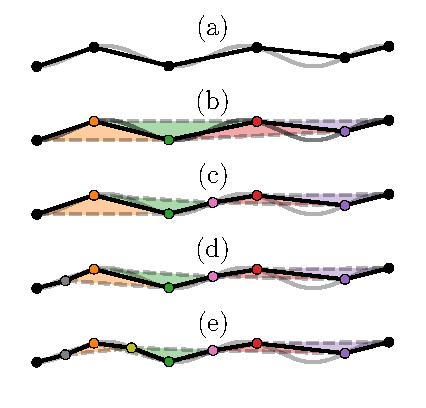
\includegraphics{figures/line_loss.pdf}
\caption{Line loss visualization.
In this example, we start with 6 points (a) on the function (grey).
Ignoring the endpoints, the effective area of each point is determined by its associated triangle (b).
The loss of each interval can be computed by taking the average area of the adjacent triangles.
Subplots (c), (d), and (e) show the subsequent interations following (b).}\label{fig:line_loss}
}
\end{figure}

In order to compare sampling strategies, we need to define some error.
We construct a linear interpolation function \(\tilde{f}\), which is an approximation of \(f\).
We calculate the error in the \(L^{1}\)-norm, defined as,
\[
\text{Err}_{1}(\tilde{f})=\left\Vert \tilde{f}-f\right\Vert _{L^{1}}=\int_{a}^{b}\left|\tilde{f}(x)-f(x)\right|\text{d}x.
\]
This error approaches zero as the approximation becomes better.

\begin{figure}
\hypertarget{fig:line_loss_error}{%
\centering
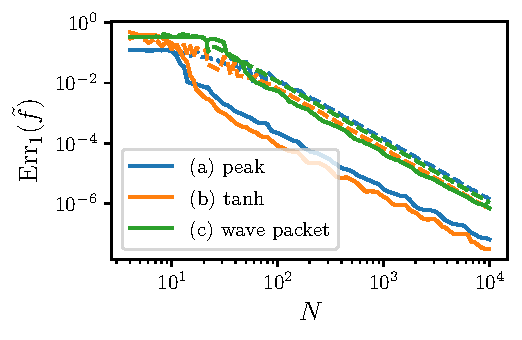
\includegraphics{figures/line_loss_error.pdf}
\caption{The \(L^{1}\)-norm error as a function of number of points \(N\) for the functions in Fig.~\ref{fig:Learner1D} (a,b,c).
The interrupted lines correspond to homogeneous sampling and the solid line to the sampling with the line loss.
In all cases adaptive sampling performs better, where the error is a factor 1.6-20 lower for \(N=10000\).}\label{fig:line_loss_error}
}
\end{figure}

Figure \ref{fig:line_loss_error} shows this error as a function of the number of points \(N\).
Here, we see that for homogeneous sampling to get the same error as sampling with a line loss, a factor \(\approx 1.6-20\) times more points are needed, depending on the function.

\hypertarget{a-parallelizable-adaptive-integration-algorithm-based-on-cquad}{%
\subsection{A parallelizable adaptive integration algorithm based on cquad}\label{a-parallelizable-adaptive-integration-algorithm-based-on-cquad}}

\hypertarget{the-cquad-algorithm-belongs-to-a-class-that-is-parallelizable.}{%
\paragraph{\texorpdfstring{The \texttt{cquad} algorithm belongs to a class that is parallelizable.}{The cquad algorithm belongs to a class that is parallelizable.}}\label{the-cquad-algorithm-belongs-to-a-class-that-is-parallelizable.}}

In Sec.~\ref{sec:review} we mentioned the doubly-adaptive integration algorithm \passthrough{\lstinline!CQUAD!} \citep{Gonnet2010}.
This algorithm uses a Clenshaw-Curtis quadrature rules of increasing degree \(d\) in each interval \citep{Clenshaw1960}.
The error estimate is \(\sqrt{\int{\left(f_0(x) - f_1(x)\right)^2}}\), where \(f_0\) and \(f_1\) are two successive interpolations of the integrand.
To reach the desired total error, intervals with the maximum absolute error are improved.
Either (1) the degree of the rule is increased or (2) the interval is split if either the function does not appear to be smooth or a rule of maximum degree (\(d=4\)) has been reached.
All points inside the intervals can be trivially calculated in parallel; however, when there are more resources available than points, Adaptive needs to guess whether an (1) interval's should degree of the rule should be increased or (2) or the interval is split.
Here, we choose to always increase until \(d=4\), after which the interval is split.

\hypertarget{isoline-and-isosurface-sampling}{%
\subsection{isoline and isosurface sampling}\label{isoline-and-isosurface-sampling}}

We can find isolines or isosurfaces using a loss function that prioritizes intervals that are closer to the function values that we are interested in.
See Fig.~\ref{fig:isoline}.

\begin{figure}
\hypertarget{fig:isoline}{%
\centering
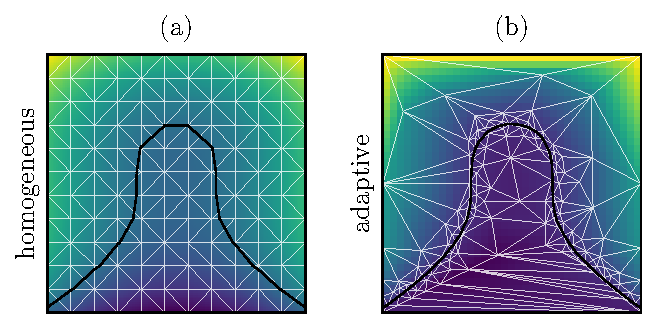
\includegraphics{figures/isoline.pdf}
\caption{Comparison of isoline sampling of \(f(x,y)=x^2 + y^3\) at \(f(x,y)=0.1\) using homogeneous sampling (left) and adaptive sampling (right) with the same amount of points \(n=17^2=289\).
We plot the function interpolated on a grid (color) with the triangulation on top (white) where the function is sampled on the vertices.
The solid line (black) indicates the isoline at \(f(x,y)=0.1\).
The isoline in the homogeneous case consists of 62 line segments and the adaptive case consists of 147 line segments.}\label{fig:isoline}
}
\end{figure}

\hypertarget{implementation-and-benchmarks}{%
\section{Implementation and benchmarks}\label{implementation-and-benchmarks}}

\hypertarget{the-learner-abstracts-a-loss-based-priority-queue.}{%
\paragraph{The learner abstracts a loss based priority queue.}\label{the-learner-abstracts-a-loss-based-priority-queue.}}

We will now introduce Adaptive's API.
The object that can suggest points based on existing data is called a \emph{learner}.
The learner abstracts a loss based priority queue.
We can either \emph{ask} it for points or \emph{tell} the \emph{learner} new data points.
We can define a \emph{learner} as follows

\begin{lstlisting}[language=Python]
from adaptive import Learner1D

def peak(x): # pretend this is a slow function
    a = 0.01
    return x + a**2 / (a**2 + x**2)

learner = Learner1D(peak, bounds=(-1, 1))
\end{lstlisting}

\hypertarget{the-runner-orchestrates-the-function-evaluation.}{%
\paragraph{The runner orchestrates the function evaluation.}\label{the-runner-orchestrates-the-function-evaluation.}}

To drive the learner manually (not recommended) and sequentially, we can do

\begin{lstlisting}[language=Python]
def goal(learner):
    # learner.loss() = max(learner.losses)
    return learner.loss() < 0.01

while not goal(learner):
    points, loss_improvements = learner.ask(n=1)
    for x in points:  # len(points) == 1
        y = f(x)
        learner.tell(x, y)
\end{lstlisting}

To do this automatically (recommended) and in parallel (by default on all cores available) use

\begin{lstlisting}[language=Python]
from adaptive import Runner
runner = Runner(learner, goal)
\end{lstlisting}

This will return immediately because the calculation happens in the background.
That also means that as the calculation is in progress, \passthrough{\lstinline!learner.data!} is accessible and can be plotted with \passthrough{\lstinline!learner.plot()!}.
Additionally, in a Jupyter notebook environment, we can call \passthrough{\lstinline!runner.live\_info()!} to display useful information.
To change the loss function for the \passthrough{\lstinline!Learner1D!} we pass a loss function, like

\begin{lstlisting}[language=Python]
def distance_loss(xs, ys): # used by default
    dx = xs[1] - xs[0]
    dy = ys[1] - ys[0]
    return np.hypot(dx, dy)

learner = Learner1D(peak, bounds=(-1, 1), loss_per_interval=distance_loss)
\end{lstlisting}

Creating a homogeneous loss function is as simple as

\begin{lstlisting}[language=Python]
def uniform_loss(xs, ys):
    dx = xs[1] - xs[0]
    return dx

learner = Learner1D(peak, bounds=(-1, 1), loss_per_interval=uniform_loss)
\end{lstlisting}

We have also implemented a \passthrough{\lstinline!LearnerND!} with a similar API

\begin{lstlisting}[language=Python]
from adaptive import LearnerND

def ring(xy): # pretend this is a slow function
    x, y = xy
    a = 0.2
    return x + np.exp(-(x**2 + y**2 - 0.75**2)**2/a**4)

learner = adaptive.LearnerND(ring, bounds=[(-1, 1), (-1, 1)])
runner = Runner(learner, goal)
\end{lstlisting}

Again, it is possible to specify a custom loss function using the \passthrough{\lstinline!loss\_per\_simplex!} argument.

\hypertarget{the-balancinglearner-can-run-many-learners-simultaneously.}{%
\paragraph{The BalancingLearner can run many learners simultaneously.}\label{the-balancinglearner-can-run-many-learners-simultaneously.}}

Frequently, more than one function (learner) needs to run at once, to do this we have implemented the \passthrough{\lstinline!BalancingLearner!}, which does not take a function, but a list of learners.
This learner internally asks all child learners for points and will choose the point of the learner that maximizes the loss improvement; thereby, it balances the resources over the different learners.
We can use it like

\begin{lstlisting}[language=Python]
from functools import partial
from adaptive import BalancingLearner

def f(x, pow):
    return x**pow

learners = [Learner1D(partial(f, pow=i)), bounds=(-10, 10) for i in range(2, 10)]
bal_learner = BalancingLearner(learners)
runner = Runner(bal_learner, goal)
\end{lstlisting}

For more details on how to use Adaptive, we recommend reading the tutorial inside the documentation \citep{Nijholt2018}.

\hypertarget{possible-extensions}{%
\section{Possible extensions}\label{possible-extensions}}

\hypertarget{anisotropic-triangulation-would-improve-the-algorithm.}{%
\paragraph{Anisotropic triangulation would improve the algorithm.}\label{anisotropic-triangulation-would-improve-the-algorithm.}}

The current implementation of choosing the candidate point inside a simplex (triangle in 2D) with the highest loss, for the \passthrough{\lstinline!LearnerND!}, works by either picking a point (1) in the center of the simplex or (2) by picking a point on the longest edge of the simplex.
The choice depends on the shape of the simplex, where the algorithm tries to create regular simplices.
Alternatively, a good strategy is choosing points somewhere on the edge of a triangle such that the simplex aligns with the gradient of the function; creating an anisotropic triangulation \citep{Dyn1990}.
This is a similar approach to the anisotropic meshing techniques mentioned in the literature review.

\hypertarget{learning-stochastic-functions-is-a-promising-direction.}{%
\paragraph{Learning stochastic functions is a promising direction.}\label{learning-stochastic-functions-is-a-promising-direction.}}

Stochastic functions frequently appear in numerical sciences.
Currently, Adaptive has a \passthrough{\lstinline!AverageLearner!} that samples a stochastic function with no degrees of freedom until a certain standard error of the mean is reached.
This is advantageous because no predetermined number of samples has to be set before starting the simulation.
Extending this learner to be able to deal with more dimensions would be a useful addition.

\hypertarget{experimental-control-needs-to-deal-with-noise-hysteresis-and-the-cost-for-changing-parameters.}{%
\paragraph{Experimental control needs to deal with noise, hysteresis, and the cost for changing parameters.}\label{experimental-control-needs-to-deal-with-noise-hysteresis-and-the-cost-for-changing-parameters.}}

Finally, there is the potential to use Adaptive for experimental control.
Experiments often deal with noise, which could be solved by taking multiple measurements and averaging over the outcomes, such as the (not yet existing) \passthrough{\lstinline!AverageLearnerND!} will do.
Another challenge in experiments is that changing parameters can be slow.
Sweeping over one dimension might be faster than in others; for example, in condensed matter physics experiments, sweeping the magnetic field is much slower than sweeping frequencies.
Additionally, some experiments exhibit hysteresis, which means that the sampling direction has to be restricted to certain paths.
All these factors have to be taken into account to create a general-purpose sampler that can be used for experiments.
However, Adaptive can already be used in experiments that are not restricted by the former effects.

\section*{Acknowledgements}
We'd like to thank \ldots{}

\section*{Author contributions statement}
Bla


\bibliographystyle{apsrev4-1}
\bibliography{paper.bib}

\end{document}
